\documentclass[a4paper]{article}

\usepackage[english]{babel}
\usepackage[utf8]{inputenc}
\usepackage{amsmath}
\usepackage{graphicx}
\usepackage[colorinlistoftodos]{todonotes}
\usepackage{hyperref}


\title{Building a Student Intervention System}

\author{Uirá Caiado}

\date{\today}

\begin{document}
\maketitle

\begin{abstract}
% it is a comment. Pretty nice, hum 
There exists a push from educators and administrators to raise the likelihood of students successfully complete their programs. The aim of this project is to identify students who need intervention before they drop out of school. My goal is to use concepts from supervised machine learning to find the most effective model with the least amount of computation costs that identify such students.
\end{abstract}

\section{Introduction}
\label{sec:introduction}

\subsection{Some Background}
As stated by \href{https://www.udacity.com/course/viewer#!/c-nd009/l-5446988865/m-5446493941}{Udacity} in the description for this project, as education has grown to rely more and more on technology, more and more data is available for examination and prediction. Logs of student activities, grades, interactions with teachers and fellow students, and more are now captured through learning management systems.

Within all levels of education, there exists a surge to help increase the likelihood of student success without watering down the education or engaging in behaviors that raise the probability of passing metrics without improving the actual underlying learning. Graduation rates are often the criteria of choice for this, and educators and administrators are after new ways to predict success and failure early enough to stage effective interventions, as well as to identify the effectiveness of different interventions.

\subsection{The Goal}
The goal for this project is implementing a student intervention system using concepts from Supervised Machine Learning. I am going to choose and develop a model that will predict the likelihood that a given student will pass, thus helping diagnose whether or not an intervention is necessary.

I will suppose that the data available to create the model is a representative but a small sample of the dataset that I would have access in the production environment. So, besides the typical accuracy requirements for any machine-learning project, I am also going to look for models that are efficient in the use of resources (computation time and memory). Thus, the model will be evaluated on three factors:

\begin{itemize}
\item Its \href{https://en.wikipedia.org/wiki/F1_score}{$F_1$} Score, summarizing the number of correct positives and correct negatives out of all possible cases. In other words, how well does the model differentiate likely passes from failures
\item The size of the training set, preferring smaller training sets over larger ones. That is, how much data does the model need to make a reasonable prediction?
\item The computation resources to make a reliable prediction. How much time and memory is required to correctly identify students that need intervention?
\end{itemize}

\subsection{Classification vs Regression}
The model that will be developed is a Classifier. According to \cite{Hastie_2009}, the distinction in the output type has led to a naming convention for prediction tasks: \textit{regression} when we predict quantitative (continuous) outputs, and \textit{classification} when we predict qualitative outputs (discrete). As the goal of this project is to identify if the student will succeed, the problem posed is a classification problem once it requires a binary answer (passed, failed).

\section{Exploring the Data}
\label{sec:exploring_data}
In this section, we will explore the data to look for insides about the features.

\subsection{Basic Facts}
Let's go ahead and execute a basic description of the student dataset (Table \ref{tab:basicfacts}):

\begin{table}[h]
\centering
\begin{tabular}{l|r}
Item & Value \\\hline
Total number of students & 42 \\
Total number of students & 395 \\
Number of students who passed & 265 \\
Number of students who failed & 130 \\
Number of features & 31 \\
Graduation rate of the class & 67.09 \%

\end{tabular}
\caption{\label{tab:basicfacts}Facts About the Dataset.}
\end{table}

All the 31 features in the dataset are discrete and Qualitative. There are 14 binary data, 13 ordered categorical variables and other 4 Categorical features. Among them, there are variables such as Father's Job, Family Size, if the student wants to take higher education or if he/she is in a romantic relationship. The data offers a pretty comprehensive profile of student life. At this point, it 's hard to say what features are relevant or not. A complete description of each variable can be found on the Github \href{https://github.com/udacity/machine-learning/tree/master/projects/student_intervention}{project page}.

Due to the nature of the data, in ``Preparing the Data'' section, the features will be coded via \href{https://www.moresteam.com/whitepapers/download/dummy-variables.pdf}{\textit{dummy variables}}. As described by \cite{Hastie_2009}, this method consists in representing a K-Level qualitative variable by a vector of K binary variables, where only one of which is ``on'' at a time. There is no missing data on this dataset and no presence of ``real'' outliers.



\subsection{How the features are spread out}
Before moving on, I am going to plot each feature to see how each inner classes of each variable are divided between the target labels ``Passed'' and ``Not Passed''. In the Figure~\ref{fig:categorical} is plotted the Categorical features of the dataset. Here is possible to see that when the guardian is not the mother nor the father, it is more likely that the pupil not pass. Also, when the mother's occupation is teaching (\textit{Fjob}), is likely that the student to pass.


\begin{figure}[h]
\centering
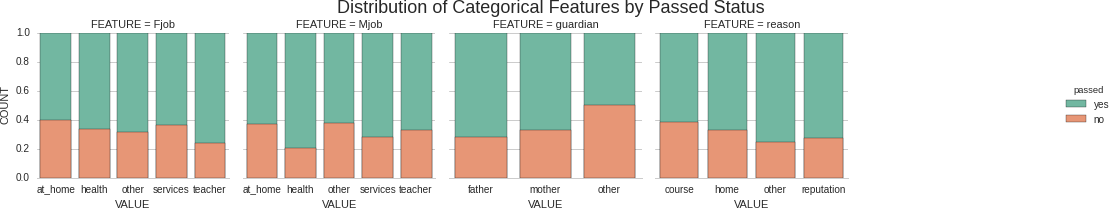
\includegraphics[width=1\textwidth]{figures/categorical/categorical.png}
\caption{\label{fig:categorical}Categorical Data.}
\end{figure}

Looking at the Ordered Categorical Features (Figure~\ref{fig:ordCategorical}), where there is an ordering of the values, the features \textit{absences}, \textit{age} and \textit{failure} stand out. The \textit{failures} feature is the number of past class failures ($n$ if $1<=n<3$, else $4$) and absences is the number of school absences. In all these variables, the bigger the number, the higher the likelihood of the student does not pass.

\begin{figure}[h]
\centering
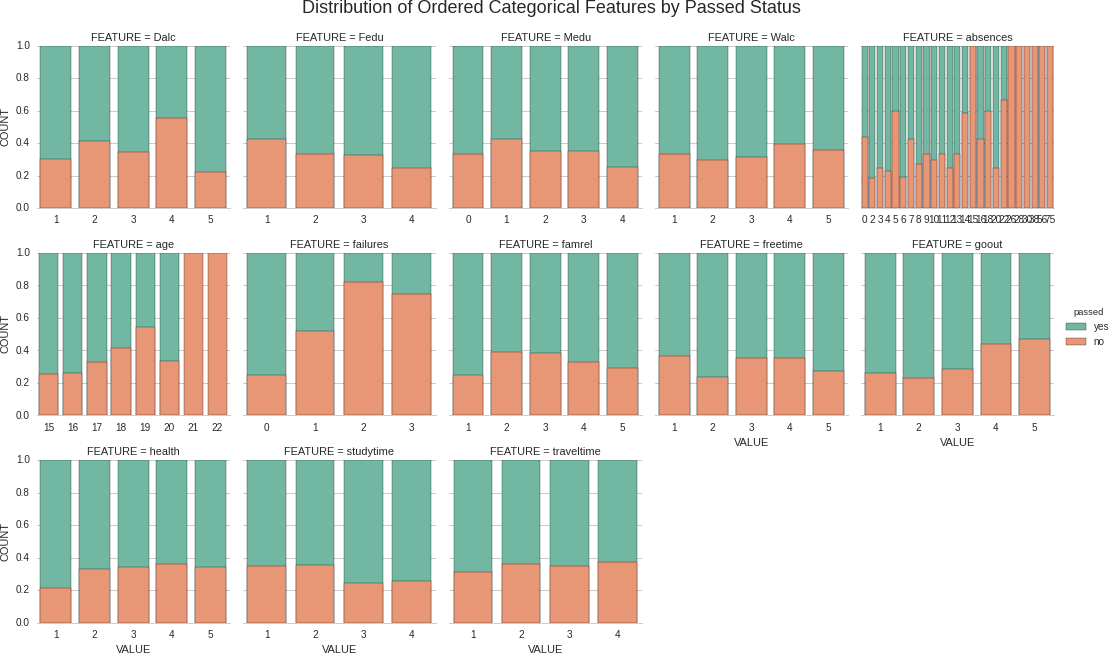
\includegraphics[width=1\textwidth]{figures/ordCategorical/ordCategorical.png}
\caption{\label{fig:ordCategorical}Ordered Data.}
\end{figure}


Finally, looking at the Binary Data (Figure~\ref{fig:binary}), what more draw the attention are the features \textit{higher} and \textit{schoolsup}. The feature \textit{higher} is if the student wants to take higher education and \textit{schoolsup} is if the student has extra educational support. Some features, as \textit{activities} and \textit{nursery}, presented a very similar distribution between the classes

\begin{figure}[h]
\centering
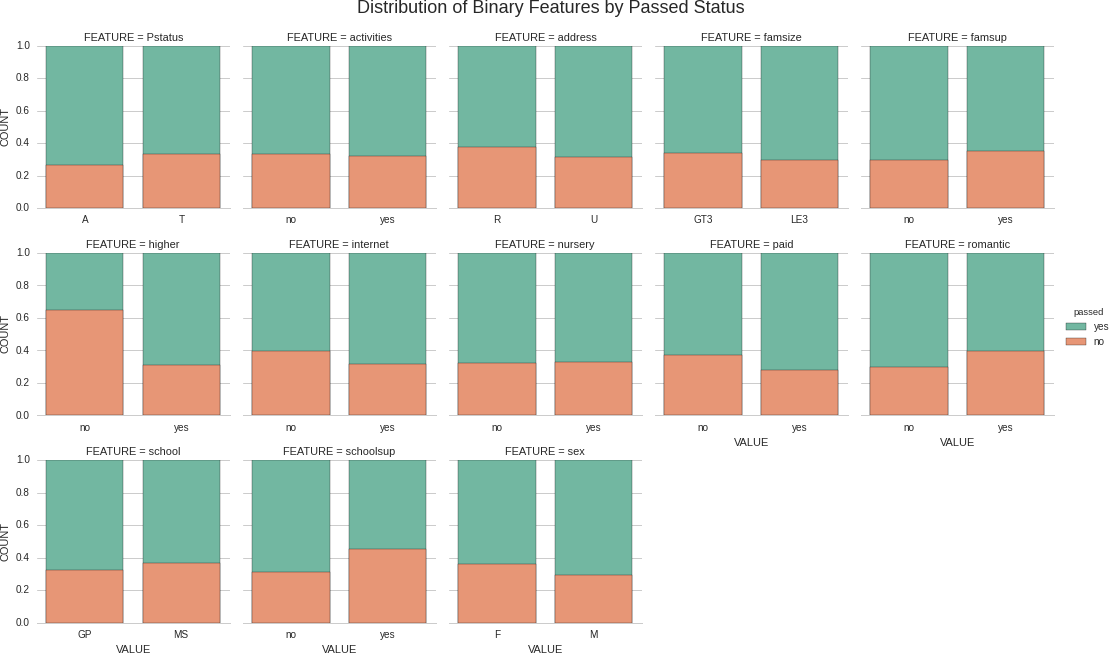
\includegraphics[width=1\textwidth]{figures/binary/binary.png}
\caption{\label{fig:binary}Binary Data.}
\end{figure}


As can be seen, there are a lot of features that might add up to the classification process, although some features may be not so relevant It is important to notice that the model developed with this amount of data (365 data points) and variables (31) can suffer from the  \href{https://en.wikipedia.org/wiki/Curse_of_dimensionality}{\textit{curse of dimensionality}}. Many of the features will be converted into dummy variables, what could increase the amount of data needed to build an accurate model. Maybe would be interesting to test if treat the binary data as numerical to reduce the necessity to split into dummies (reducing the dimension of the dataset) can increase the performance. It will be made in section 5.

\section{Preparing the Data}
In this section, we will prepare the data for modeling, training and testing.
\subsection{Identify feature and target columns}
It is often the case that the data you obtain contains non-numeric features. This can be a problem, as most machine learning algorithms expect numeric data to perform computations with.

% code snipet

\subsection{Preprocess feature columns}
...

\subsection{Split data into training and test sets}
...

\section{Training and Evaluating Models}
Show a graph of the longitudinal resistivity ($\rho_{xx}$) and Hall resistivity ($\rho_{xy}$) versus magnetic field, extracted from the raw data shown in figure \ref{fig:data}. You will have the link to the data in your absalon messages, if not e-mail Guen (guen@nbi.dk). Explain how you calculated these values, and refer to the theory.

\subsection{Classical regime}
Calculate the sheet electron density $n_{s}$ and electron mobility $\mu$ from the data in the low-field regime, and refer to the theory in section \ref{sec:theory}. Explain how you retrieved the values from the data (did you use a linear fit?).
Round values off to 1 or 2 significant digits: 8.1643 ~= 8.2. Also, 5e-6 is easier to read than 0.000005.

!OBS: This part is optional (only if you have time left).
Calculate the uncertainty as follows: \newline $u(f(x, y, z)) = \sqrt{(\frac{\delta f}{\delta{x}} u(x))^{2} + (\frac{\delta f}{\delta{y}} u(y))^{2} + (\frac{\delta f}{\delta{z}} u(z))^{2}}$, where $f$ is the calculated value ($n_{s}$ or $\mu$), $x, y, z$ are the variables taken from the measurement and $u(x)$ is the uncertainty in x (and so on).

\section{Choosing the Best Model}
Discuss your results. Compare the two values of $n_{s}$ that you've found in the previous section. Compare your results with literature and comment on the difference. If you didn't know the value of the resistance quantum, would you be able to deduce it from your measurements? If yes/no, why?



\bibliographystyle{plain}
\bibliography{bibliography/biblio.bib}


\newpage
\section{Some LaTeX tips}
\label{sec:latex}
\subsection{How to Include Figures}

First you have to upload the image file (JPEG, PNG or PDF) from your computer to writeLaTeX using the upload link the project menu. Then use the includegraphics command to include it in your document. Use the figure environment and the caption command to add a number and a caption to your figure. See the code for Figure \ref{fig:frog} in this section for an example.

\begin{figure}[h]
\centering
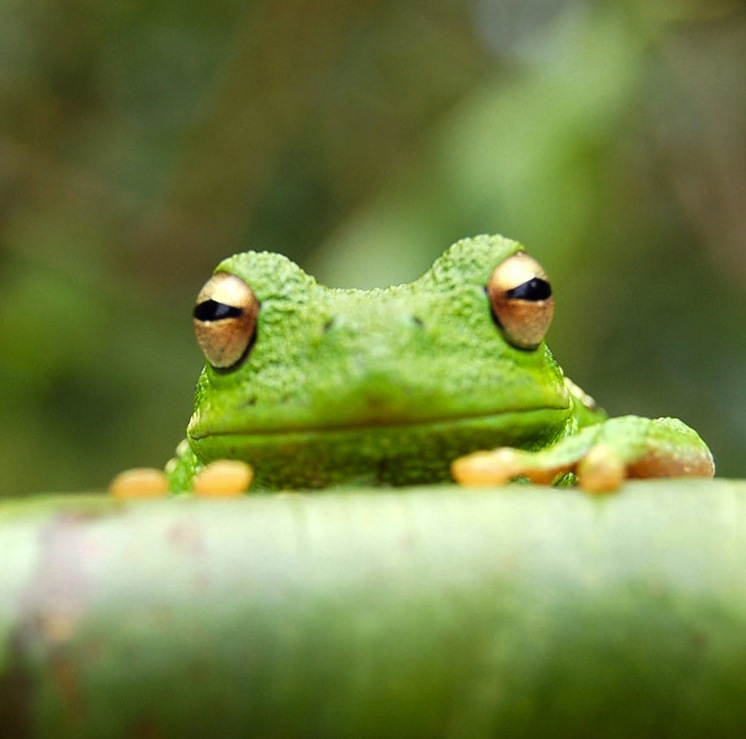
\includegraphics[width=0.3\textwidth]{frog.jpg}
\caption{\label{fig:frog}This frog was uploaded to writeLaTeX via the project menu.}
\end{figure}

\subsection{How to Make Tables}

Use the table and tabular commands for basic tables --- see Table~\ref{tab:widgets}, for example.

\begin{table}[h]
\centering
\begin{tabular}{l|r}
Item & Quantity \\\hline
Widgets & 42 \\
Gadgets & 13
\end{tabular}
\caption{\label{tab:widgets}An example table.}
\end{table}

\subsection{How to Write Mathematics}

\LaTeX{} is great at typesetting mathematics. Let $X_1, X_2, \ldots, X_n$ be a sequence of independent and identically distributed random variables with $\text{E}[X_i] = \mu$ and $\text{Var}[X_i] = \sigma^2 < \infty$, and let

\begin{equation}
S_n = \frac{X_1 + X_2 + \cdots + X_n}{n}
      = \frac{1}{n}\sum_{i}^{n} X_i
\label{eq:sn}
\end{equation}

denote their mean. Then as $n$ approaches infinity, the random variables $\sqrt{n}(S_n - \mu)$ converge in distribution to a normal $\mathcal{N}(0, \sigma^2)$.

The equation \ref{eq:sn} is very nice.

\subsection{How to Make Sections and Subsections}

Use section and subsection commands to organize your document. \LaTeX{} handles all the formatting and numbering automatically. Use ref and label commands for cross-references.

\subsection{How to Make Lists}

You can make lists with automatic numbering \dots

\begin{enumerate}
\item Like this,
\item and like this.
\end{enumerate}
\dots or bullet points \dots
\begin{itemize}
\item Like this,
\item and like this.
\end{itemize}
\dots or with words and descriptions \dots
\begin{description}
\item[Word] Definition
\item[Concept] Explanation
\item[Idea] Text
\end{description}

We hope you find write\LaTeX\ useful, and please let us know if you have any feedback using the help menu above.


\begin{thebibliography}{9}
\bibitem{nano3}
  K. Grove-Rasmussen og Jesper Nygård,
  \emph{Kvantefænomener i Nanosystemer}.
  Niels Bohr Institute \& Nano-Science Center, Københavns Universitet

\end{thebibliography}
\end{document}